%!TEX root = ../crowd_hierarchies_kdd.tex

% THIS IS AN EXAMPLE DOCUMENT FOR VLDB 2012
% based on ACM SIGPROC-SP.TEX VERSION 2.7
% Modified by  Gerald Weber <gerald@cs.auckland.ac.nz>
% Removed the requirement to include *bbl file in here. (AhmetSacan, Sep2012)
% Fixed the equation on page 3 to prevent line overflow. (AhmetSacan, Sep2012)


\section{Introduction}
\label{sec:intro}
Combining human computation with traditional computation, commonly referred to as {\em crowdsourcing}, has been recently proven beneficial in extracting knowledge and acquiring data for many application domains, including recommendation systems~\cite{amsterdamer:2014}, knowledge base completion~\cite{kondredi:2014}, entity extraction and structured data collection~\cite{park:2014,trushkowsky:2013}. In fact, extracting information, and entities in particular, from the crowd has been shown to provide access to more fine-grained information that may belong to the long tail of the web or even be completely unavailable on the web~\cite{franklin:2011, Parameswaran:2012, west:2014}.

A fundamental challenge in crowdsourced entity extraction is reasoning about the completeness of the extracted information. Given a task, e.g., ``extract all restaurants in New York'',  that seeks to extract entities from a specific domain by asking human workers, it is not easy to judge if we have extracted all entities (in this case restaurants). This is because we assume an ``open world''~\cite{franklin:2011}.

Recent work~\cite{trushkowsky:2013} has considered the problem of crowdsourced entity extraction using a single type of {\em query} that is asked to humans; for our restaurant case, the query will be ``give me another restaurant in New York''. That paper determines how many times this query must be asked to different human workers before we are sure we have extracted all restaurants in New York. However, given the monetary cost inherent in leveraging crowdsourcing, it is easy to see that just using this query repeatedly will not be practical for real-world applications, for two coupled reasons: (a) {\em wasted cost:} we will keep receiving the most popular restaurants and will have to issue many additional queries before receiving new or unseen restaurants, thus, increasing the cost; (b) {\em lack of coverage:}  beyond a point all the restaurants we get will already be present in our set of extracted entities --- thus, we may never end up receiving less popular restaurants at all.

In this paper, our goal is to {\em make crowdsourced entity extraction practical}. To do so, we focus on entity extraction over structured domains, i.e., a domain that can be fully described by a collection of attributes, each potentially displaying hierarchical structure. For example, in our restaurant case, we could have one attribute about location, one about cuisine, and one about whether the restaurant does takeout. Often the structure of domains in practical applications is already known by design. We can then leverage this structure to use a much richer space of queries asked to human workers, considering all combinations of values for each of these attributes, e.g., ``give me another Moroccan restaurant in Manhattan, New York, that does takeout''.  In this manner, we can leverage these {\em specific, targeted queries} to diversify entity extraction and obtain not-so popular entities as well.

If we view the structured data domain as a \emph{partially ordered set} (poset), then each query can be mapped to a node in the graph describing its topology. Thus, our goal is to traverse the graph corresponding to the input poset by issuing queries corresponding to various nodes, often multiple times at each node. However, the poset describing the domain can be often large, leading to many additional challenges in deciding which queries to issue at any node: (a) {\em Sparsity:} Many of the nodes in the poset are likely to be empty, i.e., the queries corresponding to those nodes are likely to not have any answers; avoiding asking queries corresponding to these nodes is essential to keep monetary cost low. (b) {\em Interrelationships:} Many of the nodes in the poset are ``coupled'' with one another; for example, the results from a few queries corresponding to ``give me another Moroccan restaurant in Manhattan, New York'' can inform whether issuing queries corresponding to ``give me another Moroccan restaurant in Manhattan, New York, that does takeout'' is useful or not. We elaborate more on these challenges in \Cref{sec:challenges} using examples from a real-world scenario.

Previously proposed techniques~\cite{trushkowsky:2013} do not directly apply to the scenario where we are traversing a poset corresponding to this structured data domain, and new techniques are needed. The main limitation of the aforementioned techniques is that they focus on estimating the completeness of a specific query and are agnostic to cost. As a consequence they do not address the problem of deciding which additional queries are \emph{worth} issuing.  To mitigate these shortcomings, one needs to tune the queries that are asked. However, deciding which queries to ask among a large number of possible queries (exponential in the number of attributes describing the input domain) and when and how many times to ask each query, are both critical challenges that need to be addressed. Furthermore, unlike previous work, we focus on the budgeted case, where we are given a budget and we want to maximize the number of retrieved entities; we believe this is a more practical goal, instead of the goal of retrieving all entities.  
\iftr
Our crowdsourced entity extraction techniques can be useful for a variety of entity extraction applications that are naturally coupled to a structured domain, including:
\squishlist
\item A newspaper that wants to collect a list of today's events to be displayed on the events page every day. 
In this case, the structured data domain could include event type (e.g., music concerts vs.~political rallies) or location, among other attributes.
\item A stock trading firm wants to collect a list of stocks that have been mentioned by popular press on the previous day. In this case, the structured data domain could include stock type, popular press article type, or whether the mention was positive or negative, among other attributes. 
\item A real estate expert wants to curate a list of houses available for viewing today. The structured data domain in this case could include the price range, the number of floors, etc.
\item A university wants to find all the faculty candidates on the job market. The structured data domain in this scenario includes the university of the applicant, specialization, and whether they are Ph.D./Postdoc.
\item The PC chair of a new conference wants to find potential reviewers. The domain describing each of the candidates can be characterized by the university or company of the reviewer, expertise, qualifications, and so on. 
\squishend
\fi

\subsection{A Real-World Scenario}
\label{sec:challenges}
To exemplify the aforementioned challenges we review a large-scale real-world scenario where crowdsourcing is used to extract entities. We consider Eventbrite~(\url{www.eventbrite.com}), an online event aggregator, that relies on crowdsourcing to compile a directory of events with detailed information about the location, type, date and category of each event. \iftr Typically, event aggregators are interested in collecting information about diverse events spanning from conferences and music festivals to political rallies across different location, i.e., countries or cities. In particular, \fi Eventbrite collects information about events across different countries in the world. Each country is split into cities and areas across the country. Moreover, events are organized according to their type and topic. The attributes and their corresponding structure are known in advance and are given by the design of the application. \iftr We collected a dataset from Eventbrite spanning over 63 countries that are divided into 1,709 subareas (e.g., states) and 10,739 cities, containing events of 19 different types, such as rallies, tournaments, conferences, conventions, etc. and a time period of 31 days spanning over the months of October and November. \fi

Two of the three dimensions, i.e., location and time, describing the domain of collected events  are hierarchically structured. The poset characterizing the domain can be fully specified if we consider the cross product across the possible values for location, event type and time. For each of the location, time, type dimensions we also consider a special {\em wildcard} value. Taking the cross-product across the possible values of these dimensions results in poset with a total of 8,508,160 nodes containing 57,805 distinct events overall. We point out that the events associated with a node in the poset overlap with the events corresponding to its descendants. First, we demonstrate how the sparsity challenge applies to Eventbrite.
\begin{example}
We plot the number of events for each node in the poset describing the Eventbrite domain. Out of 8,508,160 nodes only 175,068 nodes are associated with events while the remaining have zero events. \Cref{fig:eventbritepop} shows the number of events per node (y-axis is in log-scale). Most of the populated nodes have less than 100 events. Additionally, the most populated nodes of the domain correspond to nodes at the higher levels of the poset. When extracting events from such a sparse domain one needs to carefully decide on the crowdsourced queries to be issued especially if operating under a monetary budget.
\end{example}
\iftr
\begin{figure}
	\begin{center}
	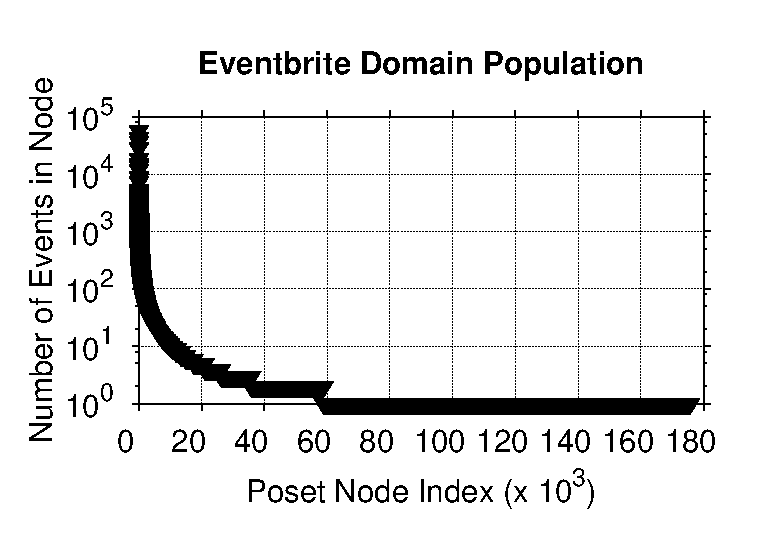
\includegraphics[clip,scale=0.5]{figs/eventbritepop.eps}
	\vspace{-10pt}
	\caption{The population of different nodes in the Eventbrite domain.}
	\label{fig:eventbritepop}
	\vspace{-10pt}
	\end{center}
\end{figure}
\fi

\ifpaper
\begin{figure}[h]
	\centering
	\vspace{-10pt}
	\subfigure{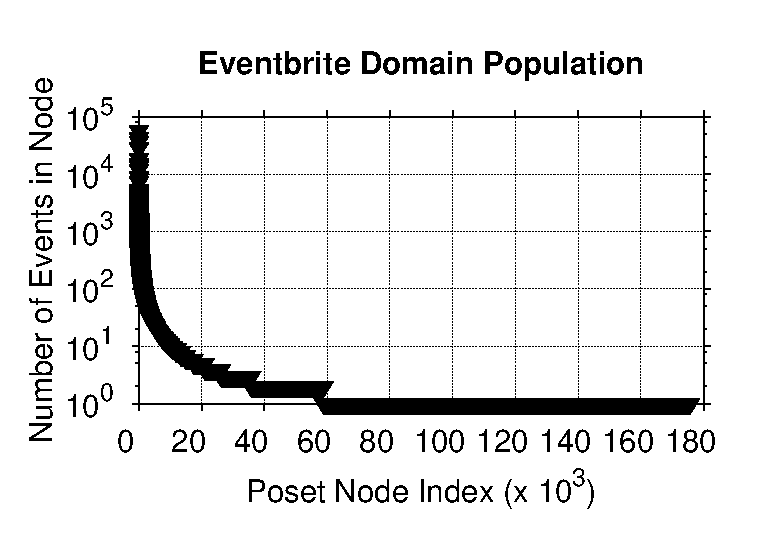
\includegraphics[clip,scale=0.32]{figs/eventbritepop.eps}\label{fig:eventbritepop}}
	\hspace{-10pt}
	\subfigure{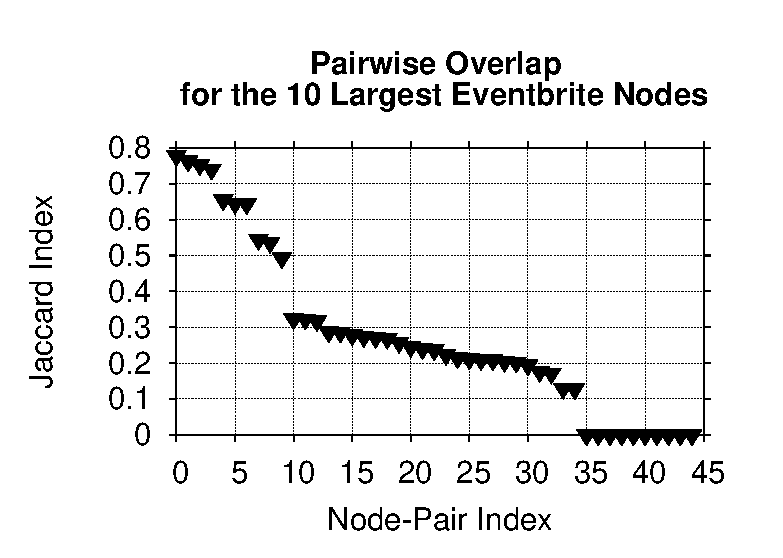
\includegraphics[clip,scale=0.32]{figs/overlaps.eps}\label{fig:eventbriteover}}
	\vspace{-10pt}
	\caption{(a) The population of different nodes and (b) pairwise overlaps for the 10 most populous nodes in the Eventbrite domain.}
	\vspace{-10pt}
\end{figure}
\fi

As mentioned before, a critical challenge in such large domains is deciding on the queries to ask. However, the hierarchical structure of the data domain presents us with an opportunity. One approach would be to perform a top-down traversal of the poset and issue queries at the different nodes. Nevertheless, this gives rise to a series of challenges: (i) how can one decide on the number of queries to be asked at each node, (ii) when should one progress to deeper levels of the poset and (iii) which subareas should be explored. We elaborate on these in \Cref{sec:prelims}. Next, we focus on the second challenge, i.e., the interdependencies across poset nodes. 
\begin{example}
We consider again the Eventbrite dataset and plot the pairwise overlaps of the ten most populous nodes in the domain. \Cref{fig:eventbriteover} shows the Jaccard index for the corresponding node pairs. As shown the event populations corresponding to these nodes overlap significantly. It is easy to see that when issuing queries at a certain domain node, we not only obtain events corresponding to this node but to other nodes in the domain as well.
\end{example}
A critical issue that stems from the overlaps across nodes is being able to decide how many answers to expect when issuing an additional query at a node whose underlying population overlaps with nodes associated with previous queries. In \Cref{sec:prelims}, we elaborate more on the dependencies across nodes of the poset.
\iftr
\begin{figure}
	\begin{center}
	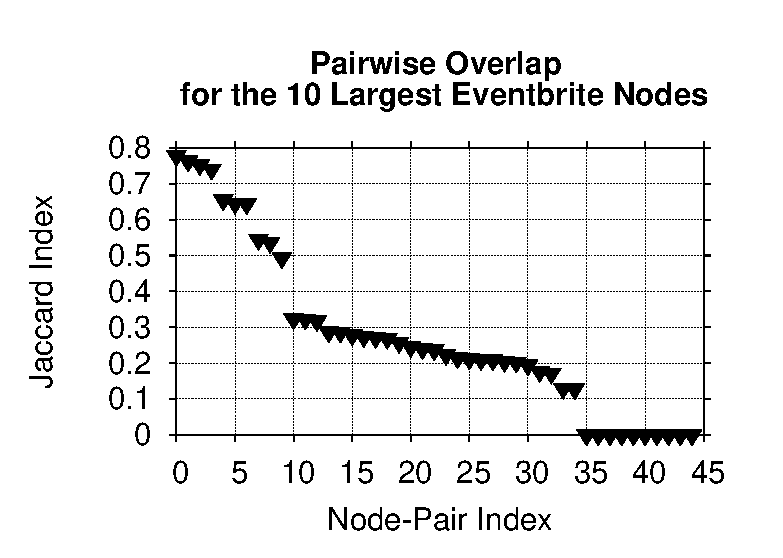
\includegraphics[clip,scale=0.5]{figs/overlaps.eps}
	\vspace{-10pt}
	\caption{Pairwise overlaps for the 10 most populous nodes.}
	\label{fig:eventbriteover}
	\vspace{-10pt}
	\end{center}
\end{figure}
\fi
\subsection{Contributions}
\label{sec:contributions}
Motivated by the examples above, we study the problem of entity extraction over {\em structured domains}. More precisely, we focus on domains described by a collection of attributes, each following a known {\em hierarchical structure}, i.e., we assume that for each attribute the corresponding hierarchy is known. Such hierarchies are usually dictated by the design of applications. \iftr Moreover, as controlling the overall extraction cost in large-scale applications is crucial we focus on {\em budgeted crowd entity extraction}. \fi

We propose a novel algorithmic framework that exploits the structure of the domain to maximize the number of extracted entities under given budget constraints. In particular, we view the problem of entity extraction as a {\em multi-round adaptive optimization problem}. At  each round we exploit the information on extracted entities obtained by previous queries to adaptively select the crowd query that will maximize the {\em cost-gain} trade-off at each round. The gain of a query is defined as the {\em number of new unique entities extracted}. 

We extend on previous query interfaces that considered only questions of the type ``Give me $k$ more entities of with attributes $\bar{X}$ that belong in domain $D$'' and examine {\em generalized queries} that can also include an {\em exclude list}. In general such queries are of the type ``Give me $k$ more entities with attributes $\bar{X}$ that belong in domain $D$ and are not in $\{A, B, ...\}$''. Extending techniques from the species estimation and building upon the multi-armed bandits literature, we introduce a new methodology for estimating the gain for such generalized queries and show how the hierarchical structure of the domain can be exploited to increase the number of extracted entities. Our main contributions are as follows:

\squishlist
\item We study the challenge of information flow across entity extraction queries for overlapping parts of the data domain.
\item We formalize the notion of an exclude list for crowdsourced entity extraction queries and show how previously proposed gain estimators can be extended to handle such queries.
\item We develop a new technique to estimate the gain of generalized entity extraction queries under the presence of little information, i.e., only when a small portion of the underlying entity population has been observed. We empirically demonstrate its effectiveness when extracting entities from sparse domains.
\item We introduce an adaptive optimization algorithm that takes as input the gain estimates for different types of queries and identifies querying policies that maximize the total number of retrieved entities under given budget constraints. 
\item Finally, we show that our techniques can effectively solve the problem of budgeted crowd entity extraction for large data domains on both real-world and synthetic data.
\squishend

